%%%%%%%%%%%%%%%%%%%% ANEXOS / APPENDIX %%%%%%%%%%%%%%%%%%%%%%
\appendix           % appendix starts from here
\appendixpage  		% add a blank page to start the appendix
\addappheadtotoc 	% add appendix to the TOC

\chapter{Reinforcement Learning}
\label{chap:appendix-c1}

\section{Classic learning methods in RL} \label{app:classic_rl}
\subsection{Monte Carlo estimation:} 
Monte Carlo estimation \cite{gerstner2021multilevel} uses complete episodes to approximate the value function using the empirical mean. The value function is based on the returns $G_t$, and since we are trying to approximate $V_{\pi}(s)$, our returns will be the statistic we will use to adjust the value of a state $S_t$. In non-stationary problems, where the environment may change over time, the value function will be incrementally updated as in equation \ref{eq:eq_mc_update}, and by the law of large numbers, if the number of times we visited a state $S$ goes close to infinity, then $V(S) = V_{\pi}(S)$ 

\begin{equation} \label{eq:eq_mc_update}
	V(S_t) \leftarrow V(S_t) + \alpha(G_t - V(S_t))
\end{equation}

Where $\alpha$ is the step-size hyper-parameter that tells the update function how much error take into account in the when performing the adjustments from the estimates. This approach has unbiased but noisy estimations, as the rewards distribution may not be consistent between episodes, creating prone-to-error estimates that may take a long time to converge to the true value function $V_{\pi}(s)$.

\subsection{Temporal Difference Learning:}
TD methods learn from episodic and non-episodic experiences, so the concept of bootstrapping is introduced. Bootstrapping refers to the ability of a model to make an approximation of the value function every each \textit{n-steps}, using the estimation of the returns we have computed as we have collected more and more experience without finishing the current episode. The simplest set-up of TD is TD(0), where we look ahead only one time-step, from $S$ to $S_{t+1}$, and the update for the value function is defined in equation \ref{eq:eq_td0_update}.

\begin{equation} \label{eq:eq_td0_update}
	V(S_t) \leftarrow V(S_t) + \alpha(R_{t+1} + \gamma V(S_{t+1}) - V(S_t))
\end{equation}

Why is this a good idea? imagine a situation where an agent is driving a car, and another car comes towards the agent, but avoids it in the last moment. In the Monte Carlo learning approach, as it learns from complete episodes, the agent would not have learned anything, since the episode ended without much consequences. In TD(0), since it is learning from each time-step, the agent would have learn from the experience itself, and for example, discover that, when a car is approaching, slowing down to have better maneuverability could be an great approach.

Looking just one step in the future might be a little short-sighted, so we can consider to look several steps ahead, considering:

\begin{itemize}
	\item For n = 1 $\rightarrow G^{1}_t = R_{t+1} + \gamma V(S_{t+1})$
	\item For n = 2 $\rightarrow G^{2}_t = R_{t+1} + \gamma R_{t+2} + \gamma V(S_{t+1})$
	\item For n = k $\rightarrow G^{k}_t = R_{t+1} + \gamma R_{t+2} ... \gamma^{k-1}R_{t+k} + \gamma^{k} V(S_{t+k})$
\end{itemize}

What we may not know which n is better, since the search space can be infinite. So the solution that TD($\lambda$) proposes is to have a weighted sum of the returns taking into account different time horizons (equation \ref{eq:lamda_return}), and then use it as our estimation of the value as portrayed in update equation \ref{eq:tdlambda_update}. Figure \ref{fig:td_returns} portrays a visual illustration of how this works.

\begin{equation}\label{eq:lamda_return}
	G^{\lambda}_{t} = (1-\lambda)\sum_{n=1}^{k} \lambda^{n-1}G^{n}_{t}
\end{equation}

\begin{equation} \label{eq:tdlambda_update}
	V(S_t) \leftarrow V(S_t) + \alpha(G^{\lambda}_{t} - V(S_t))
\end{equation}

A few things to comment about the TD($\lambda$) equation is that if $k=\infty$, then we would be in a similar to Monte Carlo learning update, but if $k=1$, then we would end up in the TD(0) update equation.

\begin{figure}[!h]
	\centering
	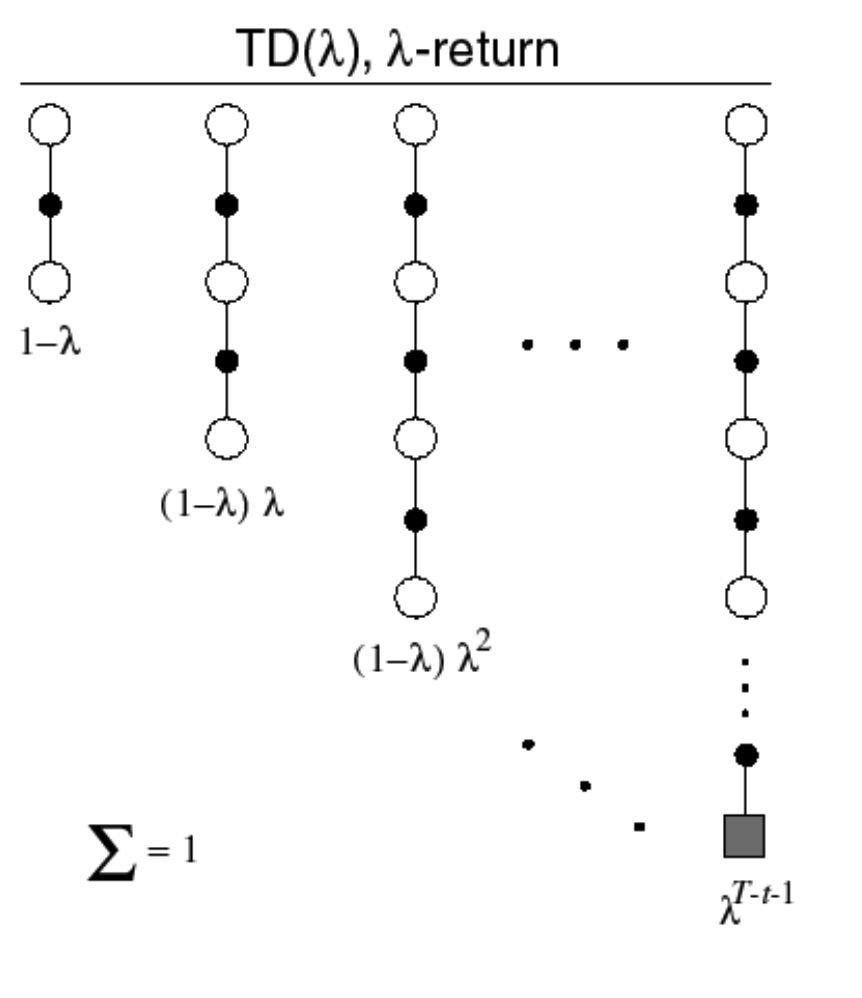
\includegraphics[scale=0.5]{figures/tdlambda_return.png}
	\caption{TD Returns}
	\label{fig:td_returns}
\end{figure}

The policy will use these values to act greedily, as defined in equation \ref{eq:eq_greedy_policy}. Since what it wants to maximize is the value, given the MDP model and the action space $\mathcal{A}$, the policy will select the action that gives more value in future states s'. The issue is that, as stated at the beginning of this section, we are in model-free RL and we no longer have the environment dynamics and $\mathcal{P}$ and reward function $\mathcal{A}$. In the next section we will introduce control, and with it, how the policy problem in tackled.

\begin{equation} \label{eq:eq_greedy_policy}
	\pi'(s) = \operatorname*{argmax}_{a \ni \mathcal{A}} \mathcal{R}^{a}_{s} + \mathcal{P}^{a}_{ss'} V(s')
\end{equation}

\subsection{On-Policy Control: } \label{app:on-policy-control}

On policy RL means that the updates of the value functions are performed according to following a policy $\pi$. Up until this point, everything we have done is evaluate states, and act according to those values. The issue is, that the policy defined in equation \ref{eq:eq_greedy_policy} requires a model of the MDP, and since we are in model-free RL, this is not possible. Instead, we introduce action-value functions, $Q(s,a)$ that take into account, the value of an action, given a state (equation \ref{eq:q_value}).

\begin{equation} \label{eq:q_value}
	q_{\pi}(s,a) = \mathbb{E}_{\pi}[R_{t+1} + \gamma q_{\pi}(S_{t+1},A_{t+1}) | S_t=s , A_t=a]
\end{equation}

Now, we re-write the policy in equation \ref{eq:action_value_policy}, that it still greedy, since we pick the action a that maximizes the action value estimates $Q$, given a state s.

\begin{equation} \label{eq:action_value_policy}
	\pi'(s) = \operatorname*{argmax}_{a \ni \mathcal{A}} {Q}(s,a)
\end{equation}

One thing to note is that, if our policy always acts greedily, then it will never explore other states, since it will always prioritize rewards over landing on new states that may lead to biggest rewards. This is why the $\epsilon$-greedy policy was introduced. This policy acts greedily with a probability of $p = (1 - \epsilon)$ and randomly with a probability $p = \epsilon$. 

Since now we are dealing with action-value functions, we must adapt the TD algorithm. This adaptation is the SARSA algorithm (State-Action-Reward-State-Action) and its update function is shown in equation \ref{eq:sarsa}.

\begin{equation} \label{eq:sarsa}
	{Q}(S,A) \leftarrow {Q}(S,A) + \alpha(R + \gamma{Q}(S',A') - {Q}(S,A))
\end{equation}

\noindent where we define the TD error in equation \ref{eq:td_error}.
\begin{equation} \label{eq:td_error}
	\delta = R + \gamma{Q}(S',A') - {Q}(S,A)
\end{equation}

If we take the approach of TD($\lambda$), we can use SARSA as a along a n-step action-value estimator, instead of just one look-ahead estimator. 

\begin{itemize}
	\item For n = 1 $\rightarrow q^{1}_t = R_{t+1} + \gamma Q(S_{t+1})$
	\item For n = 2 $\rightarrow q^{2}_t = R_{t+1} + \gamma R_{t+2} + \gamma Q(S_{t+1})$
	\item For n = k $\rightarrow q^{k}_t = R_{t+1} + \gamma R_{t+2} ... \gamma^{k-1}R_{t+k} + \gamma^{k} Q(S_{t+k})$
\end{itemize}

And using the same weighted average using the $\lambda$ parameter, we can obtain the SARSA($\lambda$) algorithm, as shown in equation \ref{eq:sarsa_lambda_return}

\begin{equation}\label{eq:sarsa_lambda_return}
	q^{\lambda}_{t} = (1-\lambda)\sum_{n=1}^{k} \lambda^{n-1}q^{n}_{t}
\end{equation}

\begin{equation} \label{eq:sarsa_lambda}
	{Q}(S_t,A_t) \leftarrow {Q}(S_t,A_t) + \alpha(q^{\lambda}_{t} - {Q}(S_t,A_t))
\end{equation}

\subsection{Off-Policy Control: } \label{app:on_policy_control}

Dealing with just one policy, $\pi$, may limit the scope of learning. To put a easy example, it would be as if humans would only learn following a single philosophy. It is not a bad approach, but as we add new perspectives to our learning process, better outcomes come out of it (i.e. work, university, relationships). Off-policy learning, among other motives, was introduce to make the agent more flexible in the learning process, taking into account different perspectives and explore while learning the optimal policy. In off-policy learning, usually there are two policies: the target policy $\pi$ that is used to compute the ${Q}$ values, and the behavioural policy $\mu$, which usually has an exploratory component to it.

One of the most famous algorithms that implements off-policy learning is Q-learning \cite{Watkins1992}. It is mainly divided in three blocks:

\begin{enumerate}
	\item The next action $A_{t+1}$ is selected following the behaviour policy $\mu(A|S_t)$
	\item The alternate action A' is selected following the target policy $\pi(A|S_t)$
	\item Use the update equation (eq. \ref{eq:q_leaning}) to update the action-values ${Q}$.
\end{enumerate}

\begin{equation} \label{eq:q_leaning}
	{Q}(S_t, A_t) \leftarrow {Q}(S_t, A_t) + \alpha[R_{t+1} +  \operatorname*{max}_{a'}\gamma{Q}(S_{t+1}, a') - {Q}(S_t, A_t)]
\end{equation}

\subsection{Actor-Critic Methods}
\label{sec:ac-methods}
Currently, the most common policy gradient methods are based on actor-critic methods. The critic (action-value function) makes evaluations of the actor's actions using function approximation $\hat{{Q}}_{w}(s,a)$. The actor tries actions and optimize them in the direction the critic proposes. This is formalized in equation \ref{eq:actor-critic} where the approximation of the policy gradient takes into account the action-value function as part of the update.

\begin{equation}\label{eq:actor-critic}
	\Delta\theta_{t} = \alpha(\nabla_{\theta} log \pi_{\theta}(s,a)\hat{{Q}}_{w}(s,a))
\end{equation}

One thing to note is that in this method we have two approximators, hence, two set of parameters, w and $\theta$. The most recent actor critic methods follow this principle, but add different optimization tools to obtain more stable and robust results in the policy learning process.

\begin{itemize}
	\item Soft Actor-Critic (SAC) \cite{haarnoja2018soft}: SAC is another off-policy actor-critic algorithm that incorporates maximum entropy reinforcement learning. It maximizes the expected return while also maximizing entropy, leading to policies that are more exploratory and robust. Right now is the state-of-the-art method for policy optimization.
	\item Proximal Policy Optimization (PPO) \cite{schulman2017proximal}: PPO is an actor-critic method that addresses the limitations of previous policy gradient methods. This is done by limiting the policy update to be close to the previous policy, helping to stabilize training and preventing large policy updates which may lead to performance degradation.
	\item Deep Deterministic Policy Gradient (DDPG) \cite{lillicrap2019continuous}: DDPG is an off-policy actor-critic algorithm specifically designed for continuous action spaces. This are spaces where the set of actions may be infinte, and a greedy (max) policy do not work. It learns a deterministic policy function using deep neural networks to approximate the Q-function and the policy.
\end{itemize}

\chapter{Attention Mechanism}

\section{Understanding the attention mechanism}
\label{app:attention-mec}

The attention mechanism appeared as a learnable alignment method for the translation task. This sequence to sequence problem had a weakness in the recursive neural network set-up. Up until that point, the way this kind of problem was addressed was by using a bidirectional RNN (usually a bi-LSTM) in the encoder, that tried to compress the information from the whole sequence in the hidden state vector from the LSTM. This was done forward and backwards to then concatenate the hidden state vectors from both LSTMs into one joint vector. This is defined in equation \ref{eq:bi_hidden_vector}

\begin{equation}
	\label{eq:bi_hidden_vector}
	\textbf{h}_1, ..., \textbf{h}_t = \text{bi-RNN}(x_1, ..., x_t)
\end{equation}

where $\textbf{h}_i$ is computed like shown in equation \ref{eq:h_vector}, where the notation $\{\cdot ; \cdot\}$ represents the concatenation between two vectors.

\begin{equation}
\begin{split}
	\label{eq:h_vector}
	\overrightarrow{h_i} = RNN_{forward}(x_i) \\
	\overleftarrow{h_i}  = RNN_{backward}(x_i) \\
	\textbf{h}_i = \{\overrightarrow{h_i};\overleftarrow{h_i}\}
\end{split}
\end{equation}

After that, the encoder, usually another RNN, would use the joint vector  $\textbf{h}_i$ to "decode" the sequence into the desired output (i.e.  the translated version of the input). As one could sense, compressing the information of big sequences becomes a problem when the hidden vector is of fixed size. What the attention mechanism proposed, was a way to dynamically change the hidden vector as the sequence was processed and new context from the input was acquired.

Bahdanu \textit{et al.} used the same set-up in the encoder in \cite{bahdanau2016neural}, but introduced new modifications at the decoder to make the hidden vector change over the time-steps of the sequence. To do so, they introduced the attention block, where the context vector $\textbf{c}_t$ is computed for each time step \textit{t}. This vector represents the relationship between the current output symbol and each term that belongs to the input sequence. Details on how the context vector $\textbf{c}_t$ is computed are at equation \ref{eq:context_vector_comp}

\begin{equation}
	\label{eq:context_vector_comp}
	c_t = \sum_{j=1}^{T} \alpha_{tj} \cdot \textbf{h}_j
\end{equation}

Where $\alpha_{tj}$ is a scalar that represents the weight of the hidden state vector $ \textbf{h}_j$ over the final context vector in time-step t. As one can interpret from equation \ref{eq:context_vector_comp},  $\alpha_{t}$ contains the information for all the input tokens processed up to the j-th element, hence, it will change its values for each time-step. Also, to prevent the decoder to "look ahead" of the sequence, the inputs tokens that are after the  j-th element in the sequence will be masked, so that the attention block cannot take them into account. The computation of  $\alpha_{tj}$ is showed in equation \ref{eq:weigth_comp}, where $s_{t-1}$ is the hidden state of the decoder at time-step t-1 and $f$ is a learnable function (i.e. a neural network) that outputs the logit (or energy, as they call it in the original work) $e_{tj}$, that ponders how much correlation exists between vectors $h_j$ and $s_{t-1}$. This correlation is then normalized by using the softmax function, producing the value $\alpha_{tj}$.

\begin{equation}
	\label{eq:weigth_comp}
	\begin{split}
		\alpha_{tj} = \frac{\text{exp}(e_{tj})}{\sum_{k=1}^{T} \text{exp}(e_{tk})} \\
		e_{tj} = f(s_{t-1}, h_j)
	\end{split}
\end{equation}

Finally, after all the alignments are computed, the RNN from the decoder outputs the most probable symbol $y_t$ at the current time-step $t$ (equation \ref{eq:dec_out_probs}).

\begin{equation}
	\label{eq:dec_out_probs}
	\mathbb{P}(y_t | y_{t-1}, ..., y_1, x) = RNN_{decoder} (c_t)
\end{equation}

\section{From attention to self-attention}
\label{from_att_2_selfatt}
Results from the attention encoder decoder architecture were a leap of performance with respect to previous work, but they still failed to perform correctly as the number of tokens in the input sequence increased. To tackle this problem, Vaswani \textit{et al.} proposed a different approach. Instead of the neural network processing one token at each time-step and compressing the information in a single hidden state vector iteratively, the sequence is processed as a whole, and each of the input tokens compute how relevant the other tokens are with respect to themselves. This mechanism is called self-attention.

To implement this mechanism, the authors propose to operate with three terms, the query Q, the keys K and the values V. These values are computed by projecting the original embeddings from the input $X \in \mathbb{R}^{n \times d}$, where n is the number of tokens in the input sequence and d is the embedding dimension, to the three matrices such that $Q = XW^Q$, $K = XW^K$ and $V = XW^V$. For clarification, $W^Q, W^K$ and $W^V \in  \mathbb{R}^{d \times d_k}$, where $d_k$ represents the dimension of the new space where $X$ is projected to compute $Q, K$ and $V$.

To follow the same terminology used in section \ref{app:attention-mec}, we are going to dissect the compact form of the attention defined in equation \ref{eq:app_self_attn} into the several parts so that resembles the way that the "classic" attention mechanism is computed.

\begin{equation}
	\label{eq:app_self_attn}
	\text{Attention}(Q, K, V) = \text{softmax}\left(\frac{QK^\top}{\sqrt{d_k}}\right) V
\end{equation}

In section \ref{app:attention-mec} we explained how the context vector $c_j$ contained the compressed information of the pondered sum from all the input tokens up to the j-th element of the sequence. On a similar fashion, the self-attention mechanism computes the context vector by projecting the j-th token of the input sequence, $x_j$, into a new space using $W^V$ and then pondering it with respect to the rest of the i-th elements from the sequence by multiplying them times $\alpha_{ij}$. As in the "classic" attention, $\alpha_{ij}$ is the normalized correlation between the i-th element and the j-th, and it is done by applying the softmax function, as shown in equation \ref{eq:self_attn_weigth_comp}, but the way $e_{i\cdot}$ is computing differs.

\begin{equation}
	\label{eq:self_attn_weigth_comp}
	\begin{split}
		\alpha_{ij} = \frac{\text{exp}(e_{ij})}{\sum_{k=1}^{n} \text{exp}(e_{ik})}
	\end{split}
\end{equation}

To compute the $e_{i\cdot}$ the self-attention formula proposes the scaled-dot product as the compatibility function. This function aims to give a magnitude of how correlated are two vectors from the input, since the dot product is greater the closer two vectors are on an euclidean space. Following this principle, we assume that the tokens that are similar semantically, will be closer in the embedding space, thus producing a greater value. The "scaled" part (i.e. $\frac{1}{\sqrt{d_z}}$)tries to stabilize the softmax function in terms of saturation, by preventing the values of the vectors from getting too big. This function is showed in equation \ref{eq:com_function_self_attn}, where $\cdot$ represents the dot-product between the i-th element in the query space and the j-th element in the key space, projected by the matrix-vector multiplication of their respective query and key projection matrices.

\begin{equation}
	\label{eq:com_function_self_attn}
	e_{ij} = \frac{(x_i W^Q)\cdot(x_j W^K)}{\sqrt{d_z}}
\end{equation}

Finally, to compute the attention-pondered final values $z_i$, we will multiply the weight values $\alpha_{ij}$ by each of the elements of the input $X$ after they are projected into the value space. Finally, we add them up, hence obtaining equation \ref{eq:final_attn_weights}.

\begin{equation}
	\label{eq:final_attn_weights}
	e_{ij} = \sum_{j=1}^{n} \alpha_{ij}(x_j) W^V
\end{equation}

As a final reflection, if we pay a closer look to equations \ref{eq:weigth_comp} and \ref{eq:com_function_self_attn}, we see that the mechanism is practically the same, where $h_i$ are the keys, and $s_{t-1}$ are the queries and the operations between them are practically the same, since $h_i$ and $s_{t-1}$ are the encoded information from the sequence in the embedded space. Something similar occurs with equations \ref{eq:final_attn_weights} and \ref{eq:context_vector_comp} where the value matrix is equivalent the $h_j$ vector at the input of the decoder. Here we can see that the relationship between the attention decoder and the self-attention mechanism from the transformer model lie under the same principles, compute which parts of the input are more relevant in terms of context to produce the appropriate output.


\chapter{Attention-models code analysis}
\label{cha:attn_models_code_analysis}

\section{Attention-based models: Vision Transformer}
\label{sec:vit_transformer_imp}
The aim of this work is to test out if there is any explain-ability in the decision making that agents perform when the value function is an approximator, which is an ideal set-up for DQN learning. For this section we will discuss the implementation of the attention-based models (i.e. vision transformers) that were used to carry out our experiments. First, we will talk about the Vision Transformer, discussing about the relevant aspects involved from the intuition to the actual implementation, that we took from \cite{caron2021emerging}. 

In several implementations for the vision transformer, we see that one of the most important things is for the model to be flexible to different configurations, where the number of blocks, embedding dimension or the number of heads in the multi-head attention block changes. This leads to easier ways to try out different configurations for the training process. For this section, first we are going to go over the constructor of the model and discuss its several parts. After that we will delve in the implementation of the most relevant.

\subsection{Constructor}
The constructor of the ViT is portrayed in listing \ref{code:vit_constructor}. We can see that the class is flexible to parameterizations, since we can specify the image size, the patch size, the channel of the input or the embedding dimension. In general terms, the constructor initializes the patch embedding module. This component is in charge of taking the input image and extract the patches from the spatial coordinates while enlarging the channel dimension from in channels to the embedding dimension. After that, it declares two essential parameters for the ViT: the class token and the positional embedding, which both of them are self learnable parameters that the network adjust during training. The next main component is a sequence of ViT blocks, which are implementations of the transformer encoder which are stacked one on top of each other. Finally, we have the classification head, which maps from the embedding dimension of the class token vector to the output dimension of the network, producing the corresponding Q value of an action as an output. We would also like to notice that for this implementation to work with the DQN and DDQN algorithm, we made some minor adaptations to the code, such as adding some additional dense layers to map from the feature space to the action space.

\begin{lstlisting} [caption={ViT model initialization}, label={code:vit_constructor}]
	def __init__(self, img_size=224, patch_size=16, in_chans=3, num_classes=0, embed_dim=768, depth=12,
	num_heads=12, mlp_ratio=4., qkv_bias=False, qk_scale=None, drop_rate=0., attn_drop_rate=0.,
	drop_path_rate=0., norm_layer=nn.LayerNorm, **kwargs):
	super().__init__()
	self.num_features = self.embed_dim = embed_dim
	
	self.patch_embed = PatchEmbed(
	img_size=img_size, patch_size=patch_size, in_chans=in_chans, embed_dim=embed_dim)
	num_patches = self.patch_embed.num_patches
	
	self.cls_token = nn.Parameter(torch.zeros(1, 1, embed_dim))
	self.pos_embed = nn.Parameter(torch.zeros(1, num_patches + 1, embed_dim))
	self.pos_drop = nn.Dropout(p=drop_rate)
	
	dpr = [x.item() for x in torch.linspace(0, drop_path_rate, depth)]  # stochastic depth decay rule
	self.blocks = nn.ModuleList([
	Block(
	dim=embed_dim, num_heads=num_heads, mlp_ratio=mlp_ratio, qkv_bias=qkv_bias, qk_scale=qk_scale,
	drop=drop_rate, attn_drop=attn_drop_rate, drop_path=dpr[i], norm_layer=norm_layer)
	for i in range(depth)])
	self.norm = norm_layer(embed_dim)
	
	# Classifier head
	self.head = nn.Linear(embed_dim, num_classes) if num_classes > 0 else nn.Identity()
	
	trunc_normal_(self.pos_embed, std=.02)
	trunc_normal_(self.cls_token, std=.02)
	self.apply(self._init_weights)
\end{lstlisting}

\subsection{Patch Embedding}
The patch embedding module is of great importance, since it is what transforms the visual data into something that is "consumable" for the ViT. The code of the patch embedding is in listing \ref{code:patch_embedding}. To perform the patch projections, they use a trick leveraging the 2D convolutional operator, where they specify the filter size and the stride as the size of the patch. This ensures that the projections are non-overlapping and reduced in the spatial dimension. Additionally, since we want the channels to be projected from the \inlinecode{in\_channels} dimension to the embedding dimension, the number of filters specified in the 2D convolution operator is the same as the embedding dimension. With this trick, the implementation is more efficient and readable, providing the embedded patches from the original image.

\begin{lstlisting}[caption={Patch Embedding module}, label={code:patch_embedding}]
	class PatchEmbed(nn.Module):
	""" 
	Image to Patch Embedding
	"""
	def __init__(self, img_size=224, patch_size=16, in_chans=3, embed_dim=768):
	super().__init__()
	num_patches = (img_size // patch_size) * (img_size // patch_size)
	self.img_size = img_size
	self.patch_size = patch_size
	self.num_patches = num_patches
	
	self.proj = nn.Conv2d(in_chans, embed_dim, kernel_size=patch_size, stride=patch_size)
	
	def forward(self, x):
	B, C, H, W = x.shape
	x = self.proj(x).flatten(2).transpose(1, 2)
	return x
\end{lstlisting}

\subsection{ViT encoder block}
Once we have our embedded image, we can proceed to process it using the ViT encoder blocks. The code of a single block is depicted in listing \ref{code:vit_block_implementation}. The input of a single block is either the embedded input image of the previous block output, to which the self attention layer will be applied, or the original image embedded. We will delve into the implementation of the attention layer after, but for now, the only thing we ought to know is that the attention layer returns the input embedding pondered by the importance of each patch. After that, it applies an projection to a layer with four times the embedding dimension to then apply a dropout layer. Since these models are very deep, in the forward pass we see that a residual connection \cite{he2015deep} is implemented in lines 17 and 18, that eases the gradient flow in the back-propagation stage.

\begin{lstlisting}[caption={ViT blocks implementation}, label={code:vit_block_implementation}]
	class Block(nn.Module):
	def __init__(self, dim, num_heads, mlp_ratio=4., qkv_bias=False, qk_scale=None, drop=0., attn_drop=0.,
	drop_path=0., act_layer=nn.GELU, norm_layer=nn.LayerNorm):
	super().__init__()
	self.norm1 = norm_layer(dim)
	self.attn = Attention(
	dim, num_heads=num_heads, qkv_bias=qkv_bias, qk_scale=qk_scale, attn_drop=attn_drop, proj_drop=drop)
	self.drop_path = DropPath(drop_path) if drop_path > 0. else nn.Identity()
	self.norm2 = norm_layer(dim)
	mlp_hidden_dim = int(dim * mlp_ratio)
	self.mlp = Mlp(in_features=dim, hidden_features=mlp_hidden_dim, act_layer=act_layer, drop=drop)
	
	def forward(self, x, return_attention=False):
	y, attn = self.attn(self.norm1(x))
	if return_attention:
	return attn
	x = x + self.drop_path(y)
	x = x + self.drop_path(self.mlp(self.norm2(x)))
	return x
\end{lstlisting}

\subsection{ViT Attention Module}
The attention blocks are the core functionality of this model. The code from the implementation is in listing \ref{code:attn_block}. In the constructor of the module, we can see that to compute the dimension of each head, it divides the embedding dimension by the number of heads we are going to apply. After that, it defines the weight matrices of the query, key and value from the self-attention module. To do so, it uses another trick to reduce the number of the layer's weights, by multiplying by three the embedding dimension, and then rearranging the tensor, so the highest order dimension is the one which contains the query, key and value values of the attention layer. After that it performs the self-attention operation, according to the equation \ref{eq:attn_eq}, obtaining the pondered embeddings. Finally, it performs some additional linear projections to obtain the final embedding. One thing that is of great use from this ViT block is that, it also returns the attentions maps from the attention blocks.

\begin{lstlisting}[caption={Attention module for the ViT model}, label={code:attn_block}]
	class Attention(nn.Module):
	def __init__(self, dim, num_heads=8, qkv_bias=False, qk_scale=None, attn_drop=0., proj_drop=0.):
	super().__init__()
	self.num_heads = num_heads
	head_dim = dim // num_heads
	self.scale = qk_scale or head_dim ** -0.5
	
	self.qkv = nn.Linear(dim, dim * 3, bias=qkv_bias)
	self.attn_drop = nn.Dropout(attn_drop)
	self.proj = nn.Linear(dim, dim)
	self.proj_drop = nn.Dropout(proj_drop)
	
	def forward(self, x):
	B, N, C = x.shape
	qkv = self.qkv(x).reshape(B, N, 3, self.num_heads, C // self.num_heads).permute(2, 0, 3, 1, 4)
	q, k, v = qkv[0], qkv[1], qkv[2]
	
	attn = (q @ k.transpose(-2, -1)) * self.scale
	attn = attn.softmax(dim=-1)
	attn = self.attn_drop(attn)
	
	x = (attn @ v).transpose(1, 2).reshape(B, N, C)
	x = self.proj(x)
	x = self.proj_drop(x)
	return x, attn
\end{lstlisting}

\subsection{The forward method}
With these main modules from the ViT explained, we can now address the \inlinecode{forward} method from the ViT class, which is portrayed in listing \ref{code:vit_forward}. First, the \inlinecode{forward} method calls \inlinecode{prepare_tokens}, which is a function that encapsulates the patch embedding functionality plus the initialization of the positional embedding and the concatenation of the token class to the patch embedding tensor, as shown in figure \ref{fig:attn_maps}. After that, the positional embedding is added to the embedded tensor, giving additional context on how the patches are arranged, to then be passed to the ViT blocks. The ViT blocks are held into a \inlinecode{ModuleList} type of object from PyTorch's library. This enables creating lists where each element is a \inlinecode{nn.Module} which can be tracked down by PyTorch's graph engine to perform forward and backward passes. The code iterates over the list of blocks, to then obtain a normalized embedding using a \inlinecode{NormLayer} module. Finally, to project from the embedding class to the action space, we perform a linear projection and obtain the class token indexing by \inlinecode{x[:, 0]}.

\begin{lstlisting}[caption={ViT forward method}, label={code:vit_forward}]
	def prepare_tokens(self, x):
	B, nc, w, h = x.shape
	x = self.patch_embed(x)  # patch linear embedding
	
	# add the [CLS] token to the embed patch tokens
	cls_tokens = self.cls_token.expand(B, -1, -1)
	x = torch.cat((cls_tokens, x), dim=1)
	
	# add positional encoding to each token
	x = x + self.interpolate_pos_encoding(x, w, h)
	
	return self.pos_drop(x)
	
	def forward(self, x):
	x = self.prepare_tokens(x)
	for blk in self.blocks:
	x = blk(x)
	x = self.norm(x)
	x = self.head(x)
	return x[:, 0]
\end{lstlisting}

\section{Attention-based models: SWIN Transformer}
\label{sec:swin_transformer_rl}
In this section we will do something similar to section \ref{sec:vit_transformer_imp}, where first we will talk about the intuition the changes with respect to the vision transformer, and then we will go over the implementation of those changes, using the code from \cite{liu2021swin}, since this model is actually more complex in the development aspect that the ViT. Another thing to note is that we will not go over the whole code used and implemented for these models, instead, we will give a comprehensive review of the implementation and delve only into the most critical aspects of them.

The SWIN transformer emerged as a version of the ViT that takes into account hierarchical features, resembling the convolutional neural networks approach to solve vision problems. It is composed from different stages, that hold different blocks. Additionally, the model introduces spatial dimension reduction, which is a big change in terms of how the model interact and manipulates the data. Additionally, it introduces the concepts of windows in order to reduce the computational overhead of the self-attention operation. In listing \ref{code:swin_transformer_constructor} we show a reduced version of the original implementation. 

\subsection{Constructor}
One of the main changes that the SWIN Transformer introduces is the positional embedding, which is relative between patches, instead of absolute as the ViT. The main reason behind this is the fact that the patches are now within windows, and the attention is computed within those windows, so each patch should have some kind of notion on where the other patches inside its window are. The code for the constructor is define in listing \ref{code:swin_transformer_constructor}. First, the declaration of the SWIN layers follows exactly the same logic as the ViT, but with a minimal difference. According to figure \ref{fig:swinarchitecture} from section \ref{sec:swin-transformer} we want for each SWIN stage to have different SWIN transformer layers, and, at the end, a patch merging transformation to reduce the spatial dimension. To do so, the BasicLayer module contains a flexible set-up where parameters such as number of heads, the depth for each layer or the window size may vary depending on the stage where is declared. The implementation is also flexible to a variable number of BasicLayer layers, since it uses the \inlinecode{ModuleList} object.

\begin{lstlisting} [caption={SWIN Transformer constructor}, label={code:swin_transformer_constructor}]
	class SwinTransformer(nn.Module):
	
	def __init__(self, img_size=224, patch_size=4, in_chans=3, num_classes=1000, embed_dim=96, depths=[2, 2, 6, 2], num_heads=[3, 6, 12, 24], window_size=7, mlp_ratio=4., qkv_bias=True, qk_scale=None, drop_rate=0., attn_drop_rate=0., drop_path_rate=0.1,	norm_layer=nn.LayerNorm, ape=False, patch_norm=True, use_checkpoint=False, **kwargs):
	super().__init__()
	
	# ... Already explained variables in VIT transformer + Patch Embedding
	
	# absolute position embedding
	if self.ape:
	self.absolute_pos_embed = nn.Parameter(torch.zeros(1, num_patches, embed_dim))
	trunc_normal_(self.absolute_pos_embed, std=.02)
	
	# ... Already explained variables in VIT transformer
	
	# build layers
	self.layers = nn.ModuleList()
	for i_layer in range(self.num_layers):
	layer = BasicLayer(dim=int(embed_dim * 2 ** i_layer),
	input_resolution=(patches_resolution[0] // (2 ** i_layer),
	patches_resolution[1] // (2 ** i_layer)),
	depth=depths[i_layer],
	num_heads=num_heads[i_layer],
	window_size=window_size,
	mlp_ratio=self.mlp_ratio,
	qkv_bias=qkv_bias, qk_scale=qk_scale,
	drop=drop_rate, attn_drop=attn_drop_rate,
	drop_path=dpr[sum(depths[:i_layer]):sum(depths[:i_layer + 1])],
	norm_layer=norm_layer,
	downsample=PatchMerging if (i_layer < self.num_layers - 1) else None,
	use_checkpoint=use_checkpoint)
	self.layers.append(layer)
	
	# ... Already explained variables in VIT transformer
	
	self.apply(self._init_weights)
\end{lstlisting}

\subsection{BasicLayer}
The \inlinecode{BasicLayer} module, defined in listing \ref{code:swin_basic_layer}, has inside of it the functionality that goes inside of every stage of the SWIN transformer. To do so, the class attribute \inlinecode{self.blocks} is declared as a \inlinecode{ModuleList} where the \inlinecode{SwinTransformerBlock} instances are declared. Since at the end of some stages, the patch merging module is applied, the \inlinecode{down\_sample} boolean flag indicates whether that stage performs down-sampling via patch merging or not. The forward method is pretty straight-forward, as the code first iterates through the  \inlinecode{SwinTransformerBlock} instances and then down-samples the spatial resolution of the returned embeddings if needed.

\begin{lstlisting}[caption={BasicLayer module that encapsulates the SWIN block functionality. It is the definition of a stage of the SWIN transformer, as defined in \ref{fig:swinarchitecture}}, label={code:swin_basic_layer}]
	class BasicLayer(nn.Module):
	
	def __init__(self, dim, input_resolution, depth, num_heads, window_size,
	mlp_ratio=4., qkv_bias=True, qk_scale=None, drop=0., attn_drop=0.,
	drop_path=0., norm_layer=nn.LayerNorm, downsample=None, use_checkpoint=False):
	
	super().__init__()
	self.dim = dim
	self.input_resolution = input_resolution
	self.depth = depth
	self.use_checkpoint = use_checkpoint
	
	# build blocks
	self.blocks = nn.ModuleList([
	SwinTransformerBlock(dim=dim, input_resolution=input_resolution,
	num_heads=num_heads, window_size=window_size,
	shift_size=0 if (i % 2 == 0) else window_size // 2,
	mlp_ratio=mlp_ratio,
	qkv_bias=qkv_bias, qk_scale=qk_scale,
	drop=drop, attn_drop=attn_drop,
	drop_path=drop_path[i] if isinstance(drop_path, list) else drop_path,
	norm_layer=norm_layer)
	for i in range(depth)])
	
	# patch merging layer
	if downsample is not None:
	self.downsample = downsample(input_resolution, dim=dim, norm_layer=norm_layer)
	else:
	self.downsample = None
	
	def forward(self, x):
	for blk in self.blocks:
	if self.use_checkpoint:
	x = checkpoint.checkpoint(blk, x)
	else:
	x = blk(x)
	if self.downsample is not None:
	x = self.downsample(x)
	return x
\end{lstlisting}

\subsection{SwinTransformerBlock}
In the \inlinecode{SWINTransformerBlock} we have the core functionality of the SWIN transformer. The first part of the constructor is defined in listing \ref{code:swin_cons_part1}. We can see that the main part is the \inlinecode{WindowAttention} class, which we will explain in the following section.

\begin{lstlisting}[caption={First part of the SWIN block constructor}, label={code:swin_cons_part1}]
	def __init__(self, dim, input_resolution, num_heads, window_size=7, shift_size=0,
	mlp_ratio=4., qkv_bias=True, qk_scale=None, drop=0., attn_drop=0., drop_path=0.,
	act_layer=nn.GELU, norm_layer=nn.LayerNorm):
	super().__init__()
	self.dim = dim
	self.input_resolution = input_resolution
	self.num_heads = num_heads
	self.window_size = window_size
	self.shift_size = shift_size
	self.mlp_ratio = mlp_ratio
	if min(self.input_resolution) <= self.window_size:
	# if window size is larger than input resolution, we don't partition windows
	self.shift_size = 0
	self.window_size = min(self.input_resolution)
	assert 0 <= self.shift_size < self.window_size, "shift_size must in 0-window_size"
	
	self.norm1 = norm_layer(dim)
	self.attn = WindowAttention(
	dim, window_size=to_2tuple(self.window_size), num_heads=num_heads,
	qkv_bias=qkv_bias, qk_scale=qk_scale, attn_drop=attn_drop, proj_drop=drop)
\end{lstlisting}

After that, in the second part of the constructor, displayed in listing \ref{code:swin_cons_part2}, handles the initialization of the window shifting for the \inlinecode{WindowAttention} model, which will be of crucial importance in order to properly arrange the context of the shifted parts of the image. To do so, it creates masks, which activate several parts of the image depending on the context, following the same scheme as explained in section \ref{sec:swin-transformer}. After that, it applies the window partitioning using the created mask. The window partition basically uses a projection of the patches that fall into the window size, which will be of use when computing the window attention.

\begin{lstlisting}[caption={Second part of the SWIN block model}, label={code:swin_cons_part2}]
	self.drop_path = DropPath(drop_path) if drop_path > 0. else nn.Identity()
	self.norm2 = norm_layer(dim)
	mlp_hidden_dim = int(dim * mlp_ratio)
	self.mlp = Mlp(in_features=dim, hidden_features=mlp_hidden_dim, act_layer=act_layer, drop=drop)
	
	if self.shift_size > 0:
	# calculate attention mask for SW-MSA
	H, W = self.input_resolution
	img_mask = torch.zeros((1, H, W, 1))  # 1 H W 1
	h_slices = (slice(0, -self.window_size),
	slice(-self.window_size, -self.shift_size),
	slice(-self.shift_size, None))
	w_slices = (slice(0, -self.window_size),
	slice(-self.window_size, -self.shift_size),
	slice(-self.shift_size, None))
	cnt = 0
	for h in h_slices:
	for w in w_slices:
	img_mask[:, h, w, :] = cnt
	cnt += 1
	
	mask_windows = window_partition(img_mask, self.window_size)  # nW, window_size, window_size, 1
	mask_windows = mask_windows.view(-1, self.window_size * self.window_size)
	attn_mask = mask_windows.unsqueeze(1) - mask_windows.unsqueeze(2)
	attn_mask = attn_mask.masked_fill(attn_mask != 0, float(-100.0)).masked_fill(attn_mask == 0, float(0.0))
\end{lstlisting}

Once the main components of the class are initialized, the \inlinecode{forward} (listing \ref{code:swin_block_fwd}) reshapes the input tensor from dimensions B, L, C, where B is the batch dimension, L is the length dimension that refers to the flattened number of patches from the input (usually as a product of the spatial dimensions: height and width) and C is the channels dimension. It reshapes the input from the flattened form to its spatial counter-part in line 7, to apply the window shifting using the \inlinecode{torch.roll} operator. Once the image is shifted, the \inlinecode{window_partition} method projects a window that holds inside a specified number of patches. For each of those windows, the attention module computes the self-attention between the patches that fall into their corresponding windows. With the attention weights applied for each window, the \inlinecode{window_reverse} method merges the window projections, returning the granularity of the input to patches. Finally, the \inlinecode{torch.roll} operator performs the shifting operation but in reverse, returning the input to its original form, but with each patch pondered by the attention weights computed for its corresponding window.

\begin{lstlisting}[caption={Forward method for the SWIN Block module}, label={code:swin_block_fwd}]
	def forward(self, x):
	H, W = self.input_resolution
	B, L, C = x.shape
	assert L == H * W, "input feature has wrong size"
	
	shortcut = x
	x = self.norm1(x)
	x = x.view(B, H, W, C)
	
	# cyclic shift
	if self.shift_size > 0:
	shifted_x = torch.roll(x, shifts=(-self.shift_size, -self.shift_size), dims=(1, 2))
	else:
	shifted_x = x
	
	# partition windows
	x_windows = window_partition(shifted_x, self.window_size)  # nW*B, window_size, window_size, C
	x_windows = x_windows.view(-1, self.window_size * self.window_size, C)  # nW*B, window_size*window_size, C
	
	# W-MSA/SW-MSA
	attn_windows = self.attn(x_windows, mask=self.attn_mask)  # nW*B, window_size*window_size, C
	
	# merge windows
	attn_windows = attn_windows.view(-1, self.window_size, self.window_size, C)
	shifted_x = window_reverse(attn_windows, self.window_size, H, W)  # B H' W' C
	
	# reverse cyclic shift
	if self.shift_size > 0:
	x = torch.roll(shifted_x, shifts=(self.shift_size, self.shift_size), dims=(1, 2))
	else:
	x = shifted_x
	x = x.view(B, H * W, C)
	
	# FFN
	x = shortcut + self.drop_path(x)
	x = x + self.drop_path(self.mlp(self.norm2(x)))
	
	return x
\end{lstlisting}

\subsection{Window Attention}
\label{sec:window_attention}
The Window Attention module from the SWIN Transformer is probably what resembles the most from the ViT. The two main differences in the SWIN transformer attention are the relative positional embedding, which was first proposed for this architecture, and the masked attention which preserves the spatial context in shited scenarios. The code is displayed in \ref{code:win_attention_constructor}. From lines 11 to 25 the relative positional index is initialized. The process to obtain it is quite convoluted, but the main intuition relies on understanding that, for each window, it is important for the patches to not only know where they are in the picture, but also know where the neighbouring patches are. By giving the relative position, the model provides a richer framework to understand not only the position of a single patch, but its position with respect to the rest of the patches inside the projected window. After this, the model uses the masks to understand which part of the window patches does it need to compute the attention. The rest of the module is pretty similar to the standard self-attention code explained in the ViT.

\begin{lstlisting}[caption={Window attention module constructor}, label={code:win_attention_constructor}]
	def __init__(self, dim, window_size, num_heads, qkv_bias=True, qk_scale=None, attn_drop=0., proj_drop=0.):
	
	super().__init__()
	self.dim = dim
	self.window_size = window_size  # Wh, Ww
	self.num_heads = num_heads
	head_dim = dim // num_heads
	self.scale = qk_scale or head_dim ** -0.5
	
	# define a parameter table of relative position bias
	self.relative_position_bias_table = nn.Parameter(
	torch.zeros((2 * window_size[0] - 1) * (2 * window_size[1] - 1), num_heads))  # 2*Wh-1 * 2*Ww-1, nH
	
	# get pair-wise relative position index for each token inside the window
	coords_h = torch.arange(self.window_size[0])
	coords_w = torch.arange(self.window_size[1])
	coords = torch.stack(torch.meshgrid([coords_h, coords_w]))  # 2, Wh, Ww
	coords_flatten = torch.flatten(coords, 1)  # 2, Wh*Ww
	relative_coords = coords_flatten[:, :, None] - coords_flatten[:, None, :]  # 2, Wh*Ww, Wh*Ww
	relative_coords = relative_coords.permute(1, 2, 0).contiguous()  # Wh*Ww, Wh*Ww, 2
	relative_coords[:, :, 0] += self.window_size[0] - 1  # shift to start from 0
	relative_coords[:, :, 1] += self.window_size[1] - 1
	relative_coords[:, :, 0] *= 2 * self.window_size[1] - 1
	relative_position_index = relative_coords.sum(-1)  # Wh*Ww, Wh*Ww
	self.register_buffer("relative_position_index", relative_position_index)
	
	self.qkv = nn.Linear(dim, dim * 3, bias=qkv_bias)
	self.attn_drop = nn.Dropout(attn_drop)
	self.proj = nn.Linear(dim, dim)
	self.proj_drop = nn.Dropout(proj_drop)
	
	trunc_normal_(self.relative_position_bias_table, std=.02)
	self.softmax = nn.Softmax(dim=-1)
\end{lstlisting}

\subsection{The forward method}

With all the main modules explained, we use the \inlinecode{forward} method as an overview of the model. The code is in listing \ref{code:forward_swin}. The \inlinecode{forward_features} method handles the feature extraction from the input image to the compressed attention-weight representation that the SWIN transformer blocks output. These features go then to the output head, that maps the embedding dimension to the output dimension, in our case the actions available in the environment.

\begin{lstlisting}[caption={Forward method for the SWIN Transformer}, label={code:forward_swin}]
	def forward_features(self, x):
	x = self.patch_embed(x)
	if self.ape:
	x = x + self.absolute_pos_embed
	x = self.pos_drop(x)
	
	for layer in self.layers:
	x = layer(x)
	
	x = self.norm(x)  # B L C
	x = self.avgpool(x.transpose(1, 2))  # B C 1
	x = torch.flatten(x, 1)
	return x
	
	def forward(self, x, head=None):
	
	x = self.forward_features(x)
	x = self.head(x)
	return x
\end{lstlisting}

As we can see, the SWIN transformer is a step-up in comparison to the ViT, with more complex and efficient ways to compute and extract relevant features using attention and spatial reduction.

\chapter{Schedulers}
\label{app:gamma_proof}

\section{Gamma for the exponential equation}
As explained in section \ref{sec:digging_dqn_agent}, the equation we must solve for gamma is the following: 
\begin{equation}
	\epsilon_t = \epsilon_0 \gamma^{\lambda t}
\end{equation}

But, since we want the equation to be bounded between $\epsilon_0$ and $\epsilon_f$ in the domain $[0, N]$, so we must substitute $\epsilon_t$ by $\epsilon_f$. Additionally, since we want the value of $\epsilon_t = \epsilon_f$ when $t = N$, then we substitute it accordingly in the equation.

\begin{align}
	\epsilon_f &=  \epsilon_0 \gamma^{\lambda N} \quad \text{(Original equation)} \label{eq1} \\
	\frac{\epsilon_f}{\epsilon_0} &= \gamma^{\lambda N} \quad \text{(Divide by $\epsilon_0$ in both sides)} \label{eq2} \\
	\sqrt[\lambda N]{\frac{\epsilon_f}{\epsilon_0}} &= \gamma \quad \text{(Exponentiation in both sides by $\frac{1}{\lambda N}$ )} \label{eq3} 
\end{align}

Hence, obtaining $\gamma$ for the exponent function.

\section{Gamma for the product of exponential equation}
Introducing again the equation in \ref{sec:digging_dqn_agent}, now we must solve for gamma: 
\begin{equation}
	\epsilon_f = \epsilon_0 \prod_{i=0}^{N} \gamma^{\lambda i}
\end{equation}

\noindent Lets begin with the procedure:
\begin{align}
	\epsilon_f &= \epsilon_0 \prod_{i=0}^{N} \gamma^{\lambda i} \quad \text{(Original equation)} \label{eq4} \\
	\frac{\epsilon_f}{\epsilon_0} &= \prod_{i=0}^{N} \gamma^{\lambda i} \quad \text{(Divide by $\epsilon_0$ in both sides)} \label{eq6} \\
	\log_\gamma \left(\frac{\epsilon_f}{\epsilon_0}\right) &= \log_\gamma \left( \prod_{i=0}^{N} \gamma^{\lambda i} \right) \quad \text{(Apply logarithms to both sides)} \label{eq7} \\
	\log_\gamma \left(\frac{\epsilon_f}{\epsilon_0}\right) &= \sum_{i=0}^{N} \log_\gamma  \gamma^{\lambda i} \quad \text{(By the product property of logarithms)} \label{eq9} \\
	\log_\gamma \left(\frac{\epsilon_f}{\epsilon_0}\right) &= \sum_{i=0}^{N} \lambda i \log_\gamma \gamma \quad \text{(By the exp. property of logarithms)} \label{eq10} \\
	\log_\gamma \left(\frac{\epsilon_f}{\epsilon_0}\right) &= \sum_{i=0}^{N} \lambda i \quad \text{(Simplifying logarithms)} \label{eq11} \\
	\log_\gamma \left(\frac{\epsilon_f}{\epsilon_0}\right) &= \lambda \sum_{i=0}^{N} i \quad \text{(Taking the constant out of the sum)} \label{eq12} 
\end{align}

Let $\sum_{i=0}^{N} i = k$, then we can compute it using the general summation formula:
\begin{equation}
	\label{eq:gen_sum}
	k = \sum_{i=0}^{N} i  = n a_1 + d \frac{(n-1)n}{2}
\end{equation}

Where $n$ is the final value, $a_1$ is the first value and $d$ is the interval between the numbers of the sum. Then, by substituting \ref{eq:gen_sum} in \ref{eq12}, we get the following:
\begin{align}
	\log_\gamma \left(\frac{\epsilon_f}{\epsilon_0}\right) &= \lambda k \quad \label{eq13}
\end{align}

And by the definition of a logarithm $\log_b(x) = y \Leftrightarrow b^y = x$, we can express equation \ref{eq13} as:

\begin{align}
	\left(\frac{\epsilon_f}{\epsilon_0}\right) &= \gamma^{\lambda k} \quad \text{(Applying the definition of a logarithm)} \label{eq14} \\
	\sqrt[\lambda k]{\frac{\epsilon_f}{\epsilon_0}} &=\gamma \quad \text{(Exponentiation of both sides by $\frac{1}{\lambda k}$)} \label{eq15}
\end{align}

Hence, obtaining $\gamma$ for the product of exponents function.
